\documentclass[11pt]{article}

%%%%%%%%%%%%%%%%%%%%%%%%%%%%%%%%%%%%%%%%%%%%%%%%%%%%%%%%%%%%%%%%%%%%%%%%%%%%%%%%
\newcommand{\term}{Section 0201, Fall 2024}
\newcommand{\course}{CMSC 451}
\newcommand{\anum}{2}
\newcommand{\duedate}{Wednesday, October 2}
%%%%%%%%%%%%%%%%%%%%%%%%%%%%%%%%%%%%%%%%%%%%%%%%%%%%%%%%%%%%%%%%%%%%%%%%%%%%%%%%

\usepackage{amsmath,amsfonts,amssymb}
\usepackage{amsthm}
\usepackage[margin=1in]{geometry}
\usepackage{enumitem}
\usepackage{ifthen}
\usepackage[colorlinks]{hyperref}
\usepackage{url}\urlstyle{same}
\usepackage[vlined,linesnumbered]{algorithm2e}
\usepackage{placeins}
\usepackage{cprotect}
\usepackage{algorithmic}
\usepackage{tikz}
\usetikzlibrary{arrows,%
  petri,%
  topaths}%
\usepackage{tkz-berge}

\setlength{\parindent}{0pt}
\setlength{\parskip}{4pt}

\newcounter{totalpoints}
\newcommand{\points}[1]{\addtocounter{totalpoints}{#1}{[#1 point\ifthenelse{\equal{#1}{1}}{}{s}]}}

%%%%%%%%%%%%%%%%%%%%%%%%%%%%%%%%%%%%%%%%%%%%%%%%%%%%%%%%%%%%%%%%%%%%%%%%%%%%%%%%

\begin{document}

{\large\textbf{ASSIGNMENT \anum} \hfill \course\ (\term)}
\smallskip\\
Due by 11:59 pm on \duedate. Submit your solutions via Gradescope.

\begin{enumerate}[leftmargin=*,start=0]

%%%%%%%%%%%%%%%%%%%%%%%%%%%%%%%%%%%%%%%%%%%%%%%%%%%%%%%%%%%%%%%%%%%%%%%%%%%%%%%%

\item \emph{Collaboration.}

Indicate that you understand the course collaboration policy and have followed it when working on this assignment. List the other students with whom you discussed the problems, or else indicate that you did not discuss any problems with your classmates.

If you consulted any resources other than the textbook to help you understand how to approach a problem, list them at the end of the solution of that problem.

\hfill

I understand the course collaboration policy, and I collaborated with Omkar Pathak, Jason Zhong, and Shril Shah.

\newpage

%%%%%%%%%%%%%%%%%%%%%%%%%%%%%%%%%%%%%%%%%%%%%%%%%%%%%%%%%%%%%%%%%%%%%%%%%%%%%%%%

\item \emph{Gears.} \points{20}

Suppose you are given a configuration of $n$ circular gears. Specifically, for each pair of gears, you are told whether or not their teeth mesh, so that turning one would cause the other to turn. One of the gears has a crank on it, and you are told which one. Design an efficient algorithm that determines (i) whether it is possible to turn the crank, and if so, (ii) whether \emph{all} the gears move when the crank is turned. Prove that your algorithm is correct and determine its asymptotic running time as a function of $n$. For full credit, your algorithm should have the smallest possible asymptotic running time.

\textit{\textbf{Algorithm.}} Let us convert the context of gears to an undirected graph such that we can use traditional 
graph theory terminology. Let each gear be a vertex. Two vertices $u, v$ have an edge if gears 
the gears $u$ and $v$'s teeth mesh. The key insight in this problem is to realize that if two nodes are connected (ie. have an edge), 
the the gears must rotate in opposite directions. That is, if gear $u$ rotates clockwise and it's teeth mesh with gear $v$, then gear $v$ must rotate 
counterclockwise. In graph terms, to show (i), we must show if the graph is \text{bipartite}. 
To show (ii), we must show that the graph is bipartite and all $n$ nodes in the graph are visited. 

\hfill

\textbf{CheckGears}(\verb|arr|, \verb|gear|)

\hspace{5mm} $//$ Assume input \verb|arr| format is \verb|[(u, v, bool), |$\cdots$\verb|]| and \verb|gear| is the gear with the crank

\hspace{5mm} Let \verb|G| be an empty adjacency list graph representation

\hspace{5mm} $//$ In \verb|directions|, $-1 \to$ not yet visited, 0 $\to$ counterclockwise, 1 $\to$ clockwise

\hspace{5mm} Set \verb|directions| to a list of size $n$, initialized to \verb|-1|s

\hspace{5mm} \textbf{For} \verb|u, v, bool| in \verb|arr|

\hspace{5mm} \textbf{If} \verb|bool == True|

\hspace{10mm} \textbf{Append} \verb|u| to \verb|G[v]| and \verb|v| to \verb|G[u]|

\hspace{5mm} $//$ Start a BFS from \verb|gear|

\hspace{5mm} Let \verb|q| be a queue with the element \verb|(gear, 0)| $//$ Start with direction 0, WLOG

\hspace{5mm} \textbf{While} \verb|q| is not empty

\hspace{10mm} Set \verb|node| and \verb|dir| be the "active" node and directions popped from the end of the \verb|q|

\hspace{10mm} \textbf{If} \verb|directions[node] == -1| $//$ this gear hasn't been visited yet

\hspace{15mm} Set \verb|directions[node] = dir|

\hspace{15mm} \textbf{For} each \verb|neighbor| of gear \verb|node| $//$ Neighbors must be direction 1 - \verb|dir|

\hspace{20mm} Add the element \verb|(neigbor, 1 - dir)| to the \verb|q|

\hspace{10mm} \textbf{If} \verb|directions[node] != dir|

\hspace{15mm} \textbf{Return} (\textbf{False, False})

\hspace{5mm} \textbf{For} \verb|node| in \verb|n|

\hspace{10mm} \textbf{If} \verb|directions[node] == -1|

\hspace{15mm} \textbf{Return} (\textbf{True, False})

\hspace{5mm} \textbf{Return} (\textbf{True, True})

\hfill

\textbf{\textit{Proof of Correctness.}}
  The algorithm converts the given "edge list" similar graph representation to an adjacency list graph representation. 
  We then start a BFS starting from the gear with the crank, and without loss of generality, allow it to spin in direction $0$, which I define 
  to be counterclockwise. All neighbors of the "active" vertex during the BFS are then appended to the queue with the opposite direction. This direction in the 
  queue must be enforced, given the fixed, existing direction of the predecessor node. If later on in the BFS, we deque one of these elements from the queue and find that it is assigned 
  the opposite direction in \verb|directions| than the assigned direction in \verb|q|, then the graph cannot be bipartite, 
  and so we return (\textbf{False, False}). If the BFS completes, then we can turn the crank. To determine if all of the gears turn, 
  we simply have to check that all gears are visited in this one BFS, so iterate through \verb|directions| and check if any elements are -1. If yes,
  we return (\textbf{True, False}) else we return (\textbf{True, True}). 
  
  \hfill

  \textbf{\textit{Time Complexity.}}
  
  In this list \verb|arr| filled with 3-tuples, there are $\binom{n}{2} = \frac{n!}{(n-2)!2!} = n(n-1)/2 = \frac{1}{2}n^2 - \frac{n}{2} \implies \mathcal{O}(n^2)$. 
  The BFS is $\mathcal{O}(V + E)$, and checking if all gears were visited is $\mathcal{O}(V)$. Thus, the overall time complexity 
  of this algorithm is $\mathcal{O}(n^2)$. 

\newpage
%%%%%%%%%%%%%%%%%%%%%%%%%%%%%%%%%%%%%%%%%%%%%%%%%%%%%%%%%%%%%%%%%%%%%%%%%%%%%%%%

\item \emph{Touring a DAG.} \points{20}

Given a directed acyclic graph $G=(V,E)$, your goal is to determine whether there is a \emph{tour} of $G$, i.e., a path that visits each vertex exactly once. If there is such a path, your algorithm should find it. Prove that your algorithm is correct and analyze its asymptotic running time as a function of $n=|V|$ and $m=|E|$. For full credit, your algorithm should run in time $O(m+n)$.

\hfill

\textbf{\textit{Algorithm.}}

\textbf{CheckTour}(\verb|V, E|)

\hspace{5mm} Set \verb|T| to \textbf{TopologicalSort}(\verb|V, E|)

\hspace{5mm} Set \verb|G| be a $V \times V$ adjacency mattrix initialized with $0$s

\hspace{5mm} \textbf{For} \verb|u, v| in \verb|E|

\hspace{10mm} Set \verb|G[u][v]| = 1

\hspace{5mm} Set \verb|i| = 0

\hspace{5mm} \textbf{While} \verb|i < V| $-1$

\hspace{10mm} \textbf{If} \verb|G[T[i]][T[i+1]]| != 1

\hspace{15mm} Return (\textbf{False}, \textbf{NULL})

\hspace{10mm} Increment \verb|i = i + 1|

\hspace{5mm} Return (\textbf{True}, \verb|T|)

\begin{proof}[\textbf{Proof of Correctness and Time Complexity}]
  Since the graph $G$ is a DAG, it has a topological sorting that contains all vertices in $V$. 
  This ordering ensures that vertices are sorted based on their dependencies to other vertices. After 
  getting the topological ordering $T$, \textbf{CheckTour} will iterate through all adjacement elements in $T$ and 
  check if there exists an edge between the two vertices. If this is true, then we return a tuple 
  containing \textbf{True} and the topological ordering $T$, otherwise we return \textbf{False} and NULL. 
  The time complexity of \textbf{CheckTour} is guaranteed to be $\mathcal{O}(m + n)$ because topological sort is 
  $\mathcal{O}(m + n)$, setting up the adjacency matrix is $\mathcal{O}(m)$, and the while loop is 
  $\mathcal{O}(n)$ because checking if there's an edge between two nodes given an adjacency matrix is $\mathcal{O}(1)$.
  Summing all these up, we get a running time of $\mathcal{O}(m + n)$, as desired.
\end{proof}


\newpage
%%%%%%%%%%%%%%%%%%%%%%%%%%%%%%%%%%%%%%%%%%%%%%%%%%%%%%%%%%%%%%%%%%%%%%%%%%%%%%%%

\item \emph{Dijkstra vs.\ Prim.}

Dijkstra's algorithm for finding a shortest-path tree and Prim's algorithm for finding a minimum spanning tree both effectively build the tree by adding low-weight edges, but they have different goals and need not produce the same output.
\begin{enumerate}
  \item \points{5} Give an example of a weighted, undirected graph $G$ with a designated vertex $s$ such that Dijkstra's algorithm on $G$ starting from $s$ and Prim's algorithm on $G$ starting from $s$ produce different results. (Try to make your example as simple as possible.)
  \item \points{15} Suppose that after running Prim's algorithm on $G=(V,E)$ with starting vertex $s$ and producing a minimum spanning tree $T$, you would like to check whether $T$ is also the shortest path tree in $G$ starting from $s$. You could do this using Dijkstra'a algorithm, but that would take time $O((m + n) \log n)$, where $n=|V|$ and $m=|E|$. Show (by giving an explicit algorithm) that in fact it is possible to determine whether $T$ is the shortest path tree in only $O(m+n)$ time. Your algorithm can take as input $G$ (including its edge weights), $s$, and $T$, where $T$ is represented by specifying the parent of each vertex. Prove both that your algorithm is correct and that its running time is $O(m+n)$. You can assume that all edge weights and shortest path lengths are distinct.
\end{enumerate}

\hfill

\textbf{\textit{Solution.}}

  \begin{enumerate}
    \item From left to right: the original graph, the shortest-path tree, and the minimum spanning tree,
    both generated from the source node $0$.
    \[
      
\includegraphics[width=4.5cm]{graph.png} 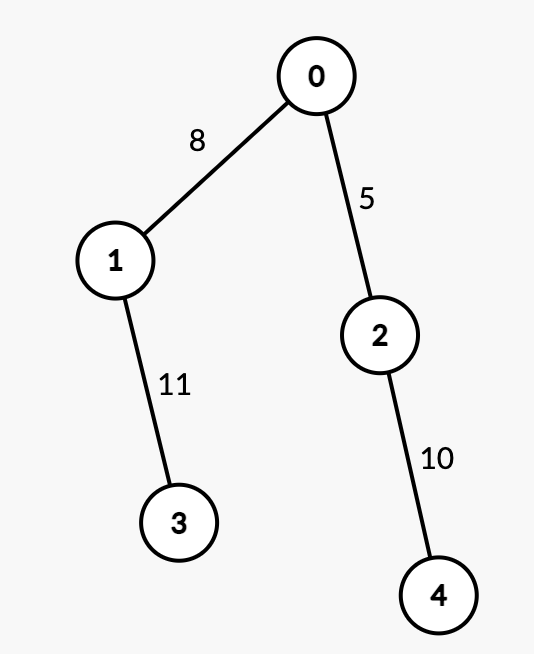
\includegraphics[width=4.5cm]{dijkstras.png} 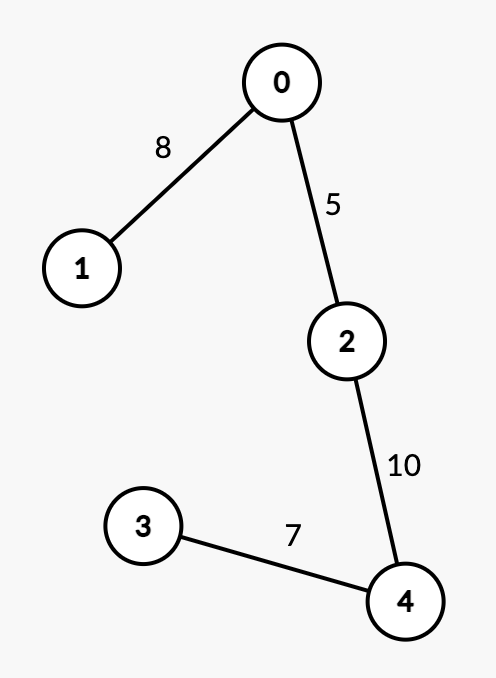
\includegraphics[width=4cm]{prims.png}
    \]
    \item Consider the following algorithm.
    
\textbf{\textit{Algorithm.}}

\textbf{ShortestPathsFromMST}(\verb|G, s, T|)

\hspace{5mm} Let \verb|dist| be a vertex-indexed array storing shortest distances from \verb|s| using edges in MST all initially initialized as $-1$

\hspace{5mm} Set \verb|dist[s] = 0|

\hspace{5mm} Let \verb|q| be a queue initialized with the starting vertex \verb|s|

\hspace{5mm} \textbf{While} \verb|q| isn't empty

\hspace{10mm} Let \verb|u| be the "active" vertex popped from \verb|q|

\hspace{10mm} \textbf{For each} neighbor \verb|v| of \verb|u| with weight \verb|w|

\hspace{15mm} \textbf{If} \verb|T[v] = u|

\hspace{20mm} Set $\verb|dist|[v] = dist[u] + w$

\hspace{20mm} Push \verb|v| into \verb|q|

\hspace{5mm} \textbf{Return} \verb|v|

\hfill

\textbf{CheckShortest}(\verb|G, s, T|)

\hspace{5mm} Set \verb|dist| = \textbf{ShortestPathsFromMST}(\verb|G, s, T|)

\hspace{5mm} Let \verb|dist2| be a vertex-indexed array storing shortest distances from \verb|s| using edges in G, all initially initialized as $-1$

\hspace{5mm} Let \verb|q2| be a queue initialized with the starting vertex \verb|s|

\hspace{5mm} Set \verb|dist2[s] = 0|

\hspace{5mm} \textbf{While} \verb|q2| isn't empty

\hspace{10mm} Pop a vertex \verb|u| from \verb|q2|

\hspace{10mm} \textbf{For each} neighbor \verb|v| of \verb|u| with weight \verb|w|

\hspace{15mm} \textbf{If} \verb|w + dist2[u] < dist[v]|

\hspace{20mm} \textbf{Return False} 

\hspace{15mm} \textbf{Else if} \verb|w + dist2[u] = dist[v]|

\hspace{20mm} Set \verb|dist2[v] = dist[v]|

\hspace{20mm} Push \verb|v| to \verb|q2|

\hspace{5mm} \textbf{Return True}
\end{enumerate}

\textbf{\textit{Proof of Correctness}}. Note that the function \textbf{ShortestPathsFromMST} correctly productes the shortest 
path from \verb|s| to all other vertices in the MST, \verb|T|. By definition of a tree, there only exists one path from any two nodes. 
Therefore, for each node $\neq$ \verb|s|, since it is the only path in the MST, it is also the shortest. The function 
\textbf{CheckShortest} correctly determines if the MST is also the shortest-path tree. By the above, \verb|dist| holds the shortest distances from 
\verb|s| to all other nodes using edges in the MST. \verb|dist2| will be similar, but can use all edges in \verb|G|. The 
algorithm begins a BFS traversal starting at \verb|s|. Now, while traversaing, we can check distances in the MST with \verb|dist|. While traversing, if we encounter a path from \verb|s| to some other node that is shorter 
than the shortest path found in the MST, then we return \textbf{False} because therefore, the MST cannot be the shortest-path tree of \verb|G|. 
At the end of the traversal, if we have visited all vertices and not exited the function by returning \textbf{False}, then we have 
essentially just followed the MST, which means the MST is the shortest-path tree and the algorithm returns \textbf{True}, as desired.

\hfill

\textbf{\textit{Time Complexity.}} Creating \verb|dist| and \verb|dist2| take $\mathcal{O}(n)$ time. \textbf{ShortestPathsFromMST}
essentially does a BFS and visited all nodes and edges, so this takes $\mathcal{O}(n + m)$ time. \textbf{CheckShortest} essentially 
does the same, so that also takes $\mathcal{O}(n + m)$ time, and vertex-lookup is always constant time because \verb|dist| and \verb|dist2| 
are vertex-indexed arrays. Therefore, the overall time complexity is $\mathcal{O}(n + m)$ time, as desired.

\newpage
%%%%%%%%%%%%%%%%%%%%%%%%%%%%%%%%%%%%%%%%%%%%%%%%%%%%%%%%%%%%%%%%%%%%%%%%%%%%%%%%

\item \emph{Scheduling to maximize profit.} \points{20}

Suppose you are given $n$ jobs, where job $i$ has deadline $d_i$ (a positive integer) and profit $p_i$ (a positive real number) for all $i \in \{1,2,\ldots,n\}$.  Each job takes unit time, so it may be scheduled in any interval $[s_i,s_i+1]$ for some nonnegative integer $s_i$ provided $s_i+1 \le d_i$ (i.e., the job is finished by its deadline) and no other job is scheduled during the same interval.  Your goal is to schedule a subset of the jobs to maximize the total profit, which is the sum of $p_i$ over all scheduled jobs $i$.  Design a greedy algorithm for this problem.  Prove that your algorithm finds an optimal schedule, and analyze its running time.

\hfill

\textbf{\textit{Algorithm.}}

\textbf{MaximizeProfit}(deadlines, profits)

\hspace{5mm} Sort the jobs in descending order s.t. $p_1 \geq p_2 \geq \cdots \geq p_n \ // $ Compute $\verb|d|_{\max}$ along the way

\hspace{5mm} Set \verb|S| be a list of size $\min(n, d_{\max})$ initialized to -1s

\hspace{5mm} Let \verb|free| be the size $\min(n, d_{\max})$ list $[1, 2, \ldots, \min(n, d_{\max})]$

\hspace{5mm} \textbf{For each} job \verb|j| in 1 to $n$

\hspace{10mm} Set $\verb|m| = \min(n, d_j) // $ Get the latest free slot $\leq \min(n, d_j)$

\hspace{10mm} \textbf{If} $\verb|m| > 0$

\hspace{15mm} Set $\verb|S|[m] = j // $ Schedule \verb|j| there

\hspace{15mm} $// $ Update \verb|free|

\hspace{15mm} \verb|m' = m|

\hspace{15mm} \textbf{While} $\verb|S[m']| \neq -1$

\hspace{20mm} \verb|free[m'] = free[m - 1]|

\hspace{20mm} Increment \verb|m' = m' + 1|

\hfill

\textit{\textbf{Proof of Correctness.} Greedy Scheduler Maximizes Profits}.
  Let $J$ be the output from the greedy algorithm, and let $S_J$ be the feasible schedule of jobs $J$. 
  Similarly, let $I$ be the output from another "optimal" algorithm, and $S_I$ is the feasible schedule of jobs $I$. 
  Note that one can rearrange $S_J \to S_J'$ and $S_I \to S_I'$ such that any $j \in I \cap J$ is done in the same slot in 
  $S_J'$ and $S_I'$. For all jobs $s \in J \cap I$

  \begin{enumerate}
    \item If $s$ in the same slot in $S_J$ and $S_I$, continue
    \item If $S_J$ schedules $s$ earlier than $S_I$, in $S_J$, swap $s$ with $t$ (where $s$ is scheduled in $S_I$). This is still feasible in $S_J$. 
    \item If $S_J$ schedules $s$ later than $S_I$, in $S_J$ do a similar swap as (b). Still feasible. 
  \end{enumerate}
  Once a job is aligned in $S_J'$ and $S_I'$, it never needs to be moved again, and we notably have that 
  \begin{align*}
    \text{profit}(S_J) = \text{profit}(S_J') && \text{profit}(S_I) = \text{profit}(S_I')
  \end{align*}

  If $S_J' \neq S_I'$, this can only happen if $J \neq I$, in which we can only have a few cases:

\begin{enumerate}
  \item Some job $s \in S_J'$ is opposite an empty slot in $S_I'$ and $s \notin I$. This contradicts the fact that $I$ is optimal, since $s$ is feasible , by definition of the $J$, the greedy set of jobs, and adding $s$ to $S_I'$ would make it more profitable. 
  \item Some job $s \in S_I'$ is opposite an empty slot in $S_J'$ and is feasible and more profitable. Therefore, $J \cup \{s\}$ is still feasible, but the greedy algorithm wouldn't have skipped it. 
  \item WLOG, suppose there's some job $s \in J$ and $t \in I$ in the same slot. If $p_s > p_t$, this contradicts the optimality of $I$. If $p_t > p_s$, the greedy algorithm skipped over $t$ to eventually choose $s$. 
  This contradicts the greediness of the algorithm. Therefore, $p_s = p_t$ is the only possibility, and so therefore
\end{enumerate}
\[\text{profit}(S_J') = \text{profit}(S_I')\]
and so the greedy algorithm outputs the optimal (most profitable) scheduling. 

\hfill

\textit{\textbf{Time Complexity}}. Sorting is $\mathcal{O}(n\log n)$, then iterating through the jobs 
and for each iteration, potentially updating \verb|free| is worst case $\mathcal{O}(n^2)$. Therefore, the overall time complexity 
of this algorithm is $\mathcal{O}(n^2)$.

\hfill

\newpage
%%%%%%%%%%%%%%%%%%%%%%%%%%%%%%%%%%%%%%%%%%%%%%%%%%%%%%%%%%%%%%%%%%%%%%%%%%%%%%%%

\item\emph{Counting significant inversions.} \points{20}

Given a list of numbers $(a_1,a_2,\ldots,a_n)$, a \emph{significant inversion} is a pair of indices $i<j$ such that $a_i>2a_j$.  Design a divide-and-conquer algorithm to count the number of significant inversions in a list of length $n$.  Prove that your algorithm is correct and analyze its running time.  For full credit, your algorithm should run in time $O(n \log n)$.

\hfill

\textbf{\textit{Algorithm.}}

\textbf{MergeSort}(arr: List, sorted: List, left: int, right: int)

\hspace{5mm} Initialize \verb|invCount = 0|

\hspace{5mm} \textbf{If} \verb|left < right|

\hspace{10mm} Set \verb|mid = floor((left + right) / 2)|

\hspace{10mm} Add \verb|invCount +=| \textbf{MergeSort}\verb|(arr, sorted, left, mid)|

\hspace{10mm} Add \verb|invCount +=| \textbf{MergeSort}\verb|(arr, sorted, mid + 1, right)|

\hspace{10mm} Add \verb|invCount +=| \textbf{Merge}\verb|(arr, sorted, left, right, mid + 1)|

\hspace{5mm} \textbf{Return} \verb|invCount|

\hfill

\textbf{Merge}(arr: List, sorted: List, left: int, right: int, mid: int)

\hspace{5mm} Set \verb|invCount| = 0

\hspace{5mm} Set \verb|i = left, j = mid, k = right| $//$ Count inversions

\hspace{5mm} \textbf{While} $\verb|i| \leq \verb|mid - 1|$ \textbf{and} $\verb|j| \leq \verb|right|$ 

\hspace{10mm} \textbf{If} \verb|arr[i] > 2 * arr[j]|

\hspace{15mm} Add \verb|invCount += (mid - i)|

\hspace{15mm} Increment \verb|j|

\hspace{10mm} \textbf{Else} increment \verb|i|

\hspace{5mm} Reset \verb|i = left, j = mid, k = right| $//$ Merge the sorted arrays

\hspace{5mm} \textbf{While} $\verb|i| \leq \verb|mid - 1|$ \textbf{and} $\verb|j| \leq \verb|right|$ 

\hspace{10mm} \textbf{If} \verb|arr[i] < arr[j]|

\hspace{15mm} Set \verb|sorted[k] = arr[i]|

\hspace{15mm} Increment \verb|i| and \verb|k|

\hspace{10mm} \textbf{Else}

\hspace{15mm} Set \verb|sorted[k] = arr[j]|

\hspace{15mm} Increment \verb|j| and \verb|k|

\hspace{5mm} $//$ Copy any remaining elements of both subarrays to \verb|sorted|

\hspace{5mm} \textbf{While} $\verb|i| \leq \verb|mid - 1|$

\hspace{15mm} Set \verb|sorted[k] = arr[i]|

\hspace{15mm} Increment \verb|i| and \verb|k|

\hspace{5mm} \textbf{While} $\verb|j| \leq \verb|right|$

\hspace{15mm} Set \verb|sorted[k] = arr[j]|

\hspace{15mm} Increment \verb|j| and \verb|k|

\hspace{5mm} $//$ Copy elements back to the original

\hspace{5mm} \textbf{For} i from \verb|left| to \verb|right + 1|

\hspace{10mm} Set \verb|arr[i] = sorted[i]|

\hspace{5mm} \textbf{Return} \verb|invCount|

\hfill

\textbf{CountInversions}(arr: List)

\hspace{5mm} Let \verb|sorted| be a list of length \verb|n|, initialized to all $0$s

\hspace{5mm} \textbf{Return MergeSort}(\verb|arr, sorted, 0, n - 1|)

\hfill

\textbf{\textit{Proof of Correctness.}} We will take the vanilla \textbf{MergeSort} and \textbf{Merge}
algorithms as already proven and only prove that the modifications in some functions yield an overall function
\textbf{CountInversions} that correctly counts the number of inversions. We will proceed with proof by induction. 

Base Case: Assume \verb|arr| is of length $1$. \textbf{MergeSort} is called and returns $0$, which is correct.

Inductive Hypothesis: Assume that \textbf{CountInversions} works correctly for list sizes $1$ to \verb|n|

Inductive Step: Note that the length of the left and right subarrays are in $[1, n]$, and so by the Inductive Hypothesis, 
\verb|invCount| after the second "Add \verb|invCount +=| $\cdots$" line is correct. The only case that we have to consider now is the number 
of significant inversions where \verb|i| is the left half of the array and \verb|j| is in the right half of the array, as all 
other cases are covered. This is in the first \textbf{While} loop in \textbf{Merge}, which follows a two pointer method. Note that both 
halves of the array are sorted by properties of \textbf{MergeSort}. If \verb|arr[i] > 2 * arr[j]|, then all elements from \verb|i|
to \verb|mid| are also significant inversions with \verb|j|, and so we add \verb|mid - i| to \verb|invCount|. In this case, we increment \verb|j| to get a
larger number in the right half of the array. Once we reach a large enough \verb|j| such that \verb|arr[i]| $\not >$ \verb|2 * arr[j]|, 
we increment \verb|i|, as there is no point incrementing \verb|j| because getting a larger \verb|arr[j]| will not make this inequality True.
This loop terminates either \verb|i| reaches \verb|mid| or \verb|j| reaches \verb|right|, and so every necessary pair has been processed, and 
\verb|invCount| correctly equals the number of significant inversions for a list of length $n + 1$. 


\hfill

\textbf{\textit{Time Complexity.}} The algorithm recursively divides lists into two halves to count the number of 
significant inversions. Note that both counting the number of inversions and merging takes $\mathcal{O}(n)$ time. Therefore, the 
recurrence relation for this algorithm can be modeled as 
\[F(n) = 2F(\frac{n}{2}) + \mathcal{O}(2n)\]
By the Master Thoerem, the time complexity for this algorithm is therefore $\mathcal{O}(n \log n)$. 


%%%%%%%%%%%%%%%%%%%%%%%%%%%%%%%%%%%%%%%%%%%%%%%%%%%%%%%%%%%%%%%%%%%%%%%%%%%%%%%%

\end{enumerate}

\end{document}
